
\chapter{Methoden und Konzepte}
\label{methoden}

\paragraph{} Um die verschiedenen genannten Anforderungen zu erfüllen, finden sich in der Literatur eine ganze Reihe von Techniken. Es würde den Rahmen dieser Arbeit sprengen, all diese Techniken vorzustellen. Um den Umfang einzuschränken gelten daher für die weitere Betrachtung folgende Einschränkungen:
\begin{enumerate}
\item Als ideale Lösung einer exakten Suche werden hier Hashing-Techniken angesehen, weil Sie das Auffinden von Suchmustern im Suchraum (nach Vorverarbeitung) in konstanter Zeit ermöglichen (siehe \cite{knuth}, S. 538).
\item Für das Problem der Teilwortsuche gelten Suffixbäume als ideale Lösung, die für ein Suchmuster der Länge $m$ und eine Anzahl von Ergebnisvorkommen $k$ das Suchproblem in $\mathcal{O}(m + k)$, also ebenfalls unabhängig von der Größe des Suchraums, lösen können (siehe \cite{gusfield}, S. 122).
\end{enumerate}
\paragraph{} Die Nutzung von Hashing und Suffixbäumen gilt also im Folgenden als gesetzt. Die weitere Auswahl von Algorithmen und Konzepten ist in den kommenden Abschnitten erläutert. Das fertige Architekturkonzept ist in Abbildung \ref{uml-architecture} im Anhang skizziert.

\section{Indizierung und Hashing}
\label{meth-hashing}

\paragraph{} Da die Benutzung von Java\texttrademark harte Voraussetzung ist (siehe \ref{intro-compatibility}) liegt die Nutzung der Hashing-Technik nahe, die die Sprache selbst bereit stellt. Java\texttrademark\\ implementiert Hashing in der Klasse \texttt{HashMap} mit Listen zur Kollisionsbehandlung und automatischem re-hashing: Bei doppelten Hashcodes werden Elemente in Eimer für den gleichen Hashcode abgelegt. Die Suchzeit vergrößert sich dabei unter Umständen leicht. Die Eimer können allerdings nicht beliebig voll werden: Ab einer Füllung der \texttt{Map} von 75\% erhöht Java\texttrademark automatisch die Größe der Tabelle und alle Einträge werden neu gehasht (siehe auch \cite{javaHashMap}). Das erfüllt die Bedingung einer konstanten Zugriffszeit hinreichend (siehe auch \cite{knuth}, S. 506-549).

\section{Suffixbäume}
\label{meth-suffix}

\paragraph{} Ein Suffixbaum für einen String $S$ der Länge $n$ ist ein gerichteter, gewurzelter Baum mit genau $n$ Blättern. Jeder Knoten im Baum, der weder Wurzel noch Blatt ist, hat wenigstens zwei Kinder und jede Kante innerhalb des Baums ist mit einem nicht-leeren Teilwort von $S$ beschrieben. Zwei Kanten, die an einem Knoten im Baum beginnen, können nicht das gleiche erste Zeichen haben. Es besteht ferner ein 1 : 1-Verhältnis zwischen den Suffixen von $S$ und den Blättern des Baumes: Für jedes Suffix $s$ von $S$ existiert genau ein Blatt $l$, so dass der Pfad von der Wurzel des Baums zu $l$ mit $s$ beschrieben ist (sinngemäß nach \cite{gusfield}, S. 90; siehe auch Abbildung \ref{fig-kehrichtSuffixTree}).

\begin{figure}
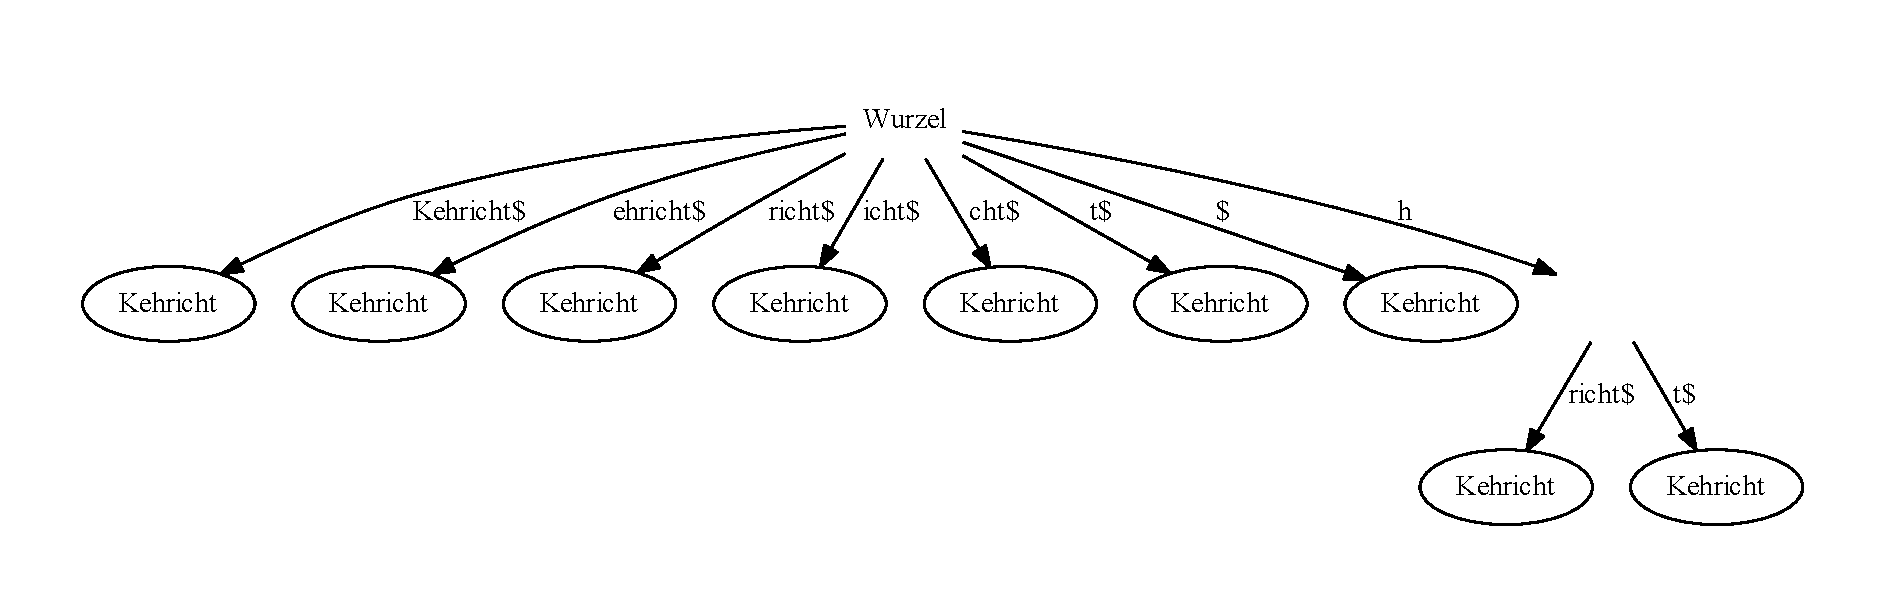
\includegraphics[scale=0.4]{resources/kehrichtSuffixTree.pdf}
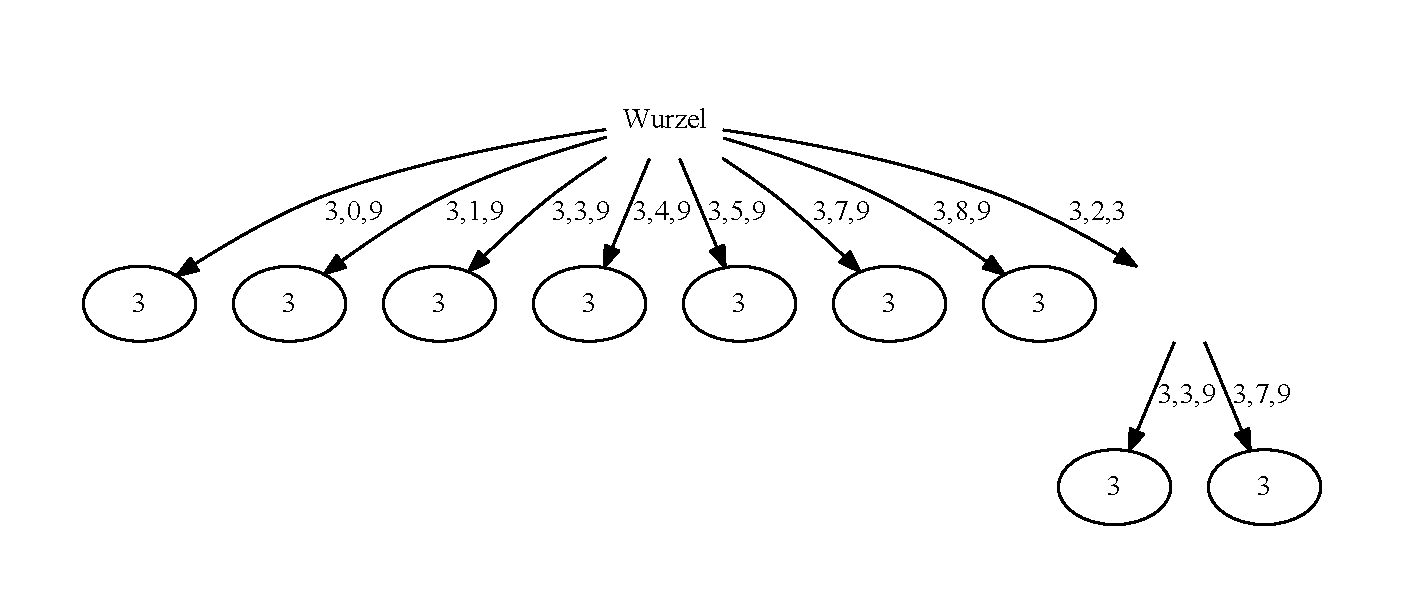
\includegraphics[scale=0.5]{resources/kehrichtCompressedSuffixTree.pdf}
\caption{\textbf{oben:} Suffixbaum  (\textit{Suffix Trie}) für das Wort "`Kehricht"'.\\\textbf{unten:} Komprimierter Suffixbaum (\textit{Suffix Tree} bzw. \textit{Compact Suffix Tree}) für das gleiche Wort. Die erste Zahl ist die ID des referenzierten Wortes, der zweite Buchstabe der Index (von 0 gezählt) des Startbuchstabens des Teilwortes, das auf dieser Kante steht und der dritte Buchstabe der Index (von 1 gezählt) des Endbuchstabens des Teilwortes, das auf der Kante steht.}
\label{fig-kehrichtSuffixTree}
\end{figure}

\paragraph{} Da Java\texttrademark keine spracheigene Implementierung eines Suffixbaumes liefert bleibt hier die Wahl des Konzepts frei. In der Literatur finden sich mehrere Vorschläge, die sich unter zwei Gesichtspunkten kategorisieren lassen:

\subsection{Aufbaualgorithmus}

\paragraph{} Die in der Literatur verbreitetsten Formen, einen Suffixbaum aufzubauen, sind die Algorithmen von Weiner, McCreight und Ukkonen in linearer Zeit (siehe auch \cite{gusfield}, S. 90). Giegerich, Kurtz und Stoye schlagen jedoch ein in der Praxis nur wenig langsameres Verfahren vor, das selbst in einer nicht-funktionellen Sprache wie Java\texttrademark lazy-evaluation\footnote{Das heißt: Die Knoten des Baumes werden erst dann evaluiert, wenn sie für eine Suchanfrage gebraucht werden und sind so lange nur implizit vorhanden.} von Suffixbäumen ermöglicht und damit deutliche Gewinne bei der Speichereffizizenz in praktischen Szenarien verspricht (siehe \cite{lazyTrees}).

\subsection{Kodierung und Kompression}

\paragraph{} Intuitiv erscheint bei der Konstruktion von Suffixbäumen eigentlich die Konstruktion eines sogenannten \textit{Suffix Trie}, also eines Suffixbaumes mit expliziten Kantenbeschriftungen (siehe auch  Definition bei Cobbs \cite{approxTreesCobbs} und Abbildung \ref{fig-kehrichtSuffixTree}, oben). Tatsächlich würde dies zu einem Speicherverbrauch von $\mathcal{O}
(n^2)$ bei einer Textlänge von $n$ führen, weshalb Techniken zur Komprimierung üblich sind. Insbesondere die Referenz auf Kantenbeschriftungen als Pointer (Edge-label-compression) ist dabei im Grunde unumstritten (siehe \cite{gusfield}, S. 104 und Abbildung \ref{fig-kehrichtSuffixTree}, unten).
Dieses Komprimierungskonzept wird auch dadurch gestützt, dass die Worte des Suchraums ohnehin für die exakte Suche in einer Hash-Tabelle indiziert werden müssen und sich daher Referenzen auf die Einträge dieser Tabelle anbieten.
\paragraph{} Weniger eindeutig allerdings ist die Lage, was weitere Komprimierungs- und Kodierungstechniken betrifft: Es erscheint auf den ersten Blick zum Beispiel naheliegend, einen Suffixbaum für den gesamten indizierten Text zu erstellen. Die genaue Reihenfolge der Worte im Text ist aber für alle Suchmodi außer der exakten Suche, die ohnehin durch Hashing gelöst werden soll, irrelevant. Demnach ist es sinnvoll, stattdessen einen generalisierten Suffixbaum zu verwenden, der nur die Worte, nicht die Vorkommen der Worte indiziert (siehe auch \cite{gusfield}, S. 116 und Abbildung \ref{fig-wolleHoldSuffixTree}).

\begin{figure}
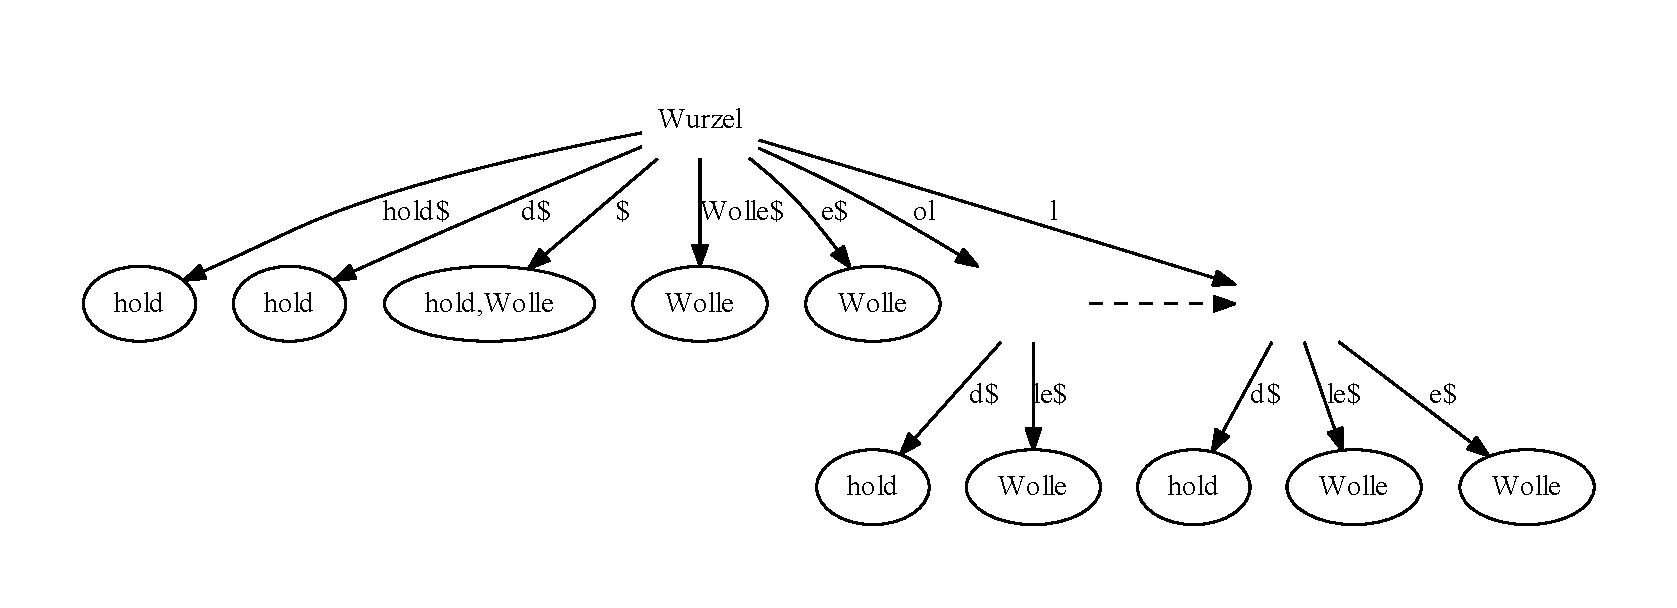
\includegraphics[scale=0.5]{resources/wolleHoldSuffixTree.pdf}
\caption{Generalisierter Suffixbaum für die Worte "`hold"' und "`Wolle"'. Für jedes Suffix beider Worte existiert je ein eindeutiger Pfad von der Wurzel zu einem Blatt, an dem alle Worte notiert sind, für die der dorthin führende Pfad ein Suffix ist. Ein Suffix-Link ist mit dem gestrichelten Pfeil angedeutet.}
\label{fig-wolleHoldSuffixTree}
\end{figure}

\paragraph{} Das allerdings erfordert Veränderungen bei zwei weiteren Konzepten: Baeza-Yates und Gonnet beschreiben das Matching von regulären Ausdrücken auf Suffixbäumen in $\mathcal{O}(n)$. Diese Technik ist nur für einen Suffixbaum über den gesamten Text beschrieben. Hier müsste außerdem der Inhalt des Suffixbaumes binär kodiert werden (siehe \cite{baeza-yates}).
\paragraph{} Ebenso verhält es sich bei der inexakten Suche: Die modernste Variante zur Lösung des Problems in Suffixbäumen (siehe Überblick in \cite{approximateIndexing}) wird von Cobbs als Weiterentwicklung eines Algorithmus von Ukkonen und Jukinen vorgestellt (siehe \cite{approxTreesUkkonen1,approxTreesUkkonen2,approxTreesCobbs}). Sie ist aber ebenfalls nur für einen Suffixbaum über den gesamten Text beschrieben.

\subsection{Auswahl des Konzepts}

\paragraph{} Die Nutzung eines Suffixbaums mit lazy evaluation erscheint zwar reizvoll, würde aber Laufzeitverluste für die Suchanfragen von Nutzenden bedeuten, weil zusätzlich zur Laufzeit der Suche die Knoten des Baums evaluiert werden müssten. Daher wird im weiteren Verlauf stattdessen der Algorithmus von Ukkonen zum Aufbau des Baumes verwendet (siehe \cite{gusfield}, S. 94-107 bzw. im Original \cite{ukkonen}).
\paragraph{} Dennoch soll durch Nutzung eines generalisierten Suffixbaums eine möglichst speichereffiziente Lösung erstellt werden. Das bedeutet jedoch, dass die vorgestellten Suchkonzepte für reguläre Ausdrücke und inexaktes Matching adaptiert werden müssen und vielleicht nur mit Einschränkungen nutzbar sind.

\section{Endliche Automaten}
\label{meth-automata}

\paragraph{} Ein endlicher Automat besteht aus einer Menge von Zuständen, zwischen denen sich der Automat je nach Eingabe bewegt. Das besondere Kennzeichen endlicher Automaten ist, dass die Folgezustände nur mittels des momentanen Zustandes und des Inputs berechnet werden können (siehe auch \cite{automata}, S. 37f.).
\paragraph{} Bei der Bearbeitung von regulären Ausdrücken schlagen Baeza-Yates und Gonnet die Nutzung von deterministischen, endlichen Automaten (DEA) vor \cite{baeza-yates}. Solche Automaten haben im Aufbau unter Umständen exponentiellen Zeit- und Platzverbrauch abhängig vom Suchmuster (siehe \cite{automata}, S. 60). Daher erscheint es wünschenswert, stattdessen auf nichtdeterministische endliche Automaten (NEA) zurückzugreifen, solange das die eigentliche Suchzeit nicht zu weit erhöht.

\section{Scoring}
\label{meth-scoring}

\paragraph{} Zwar gibt es in der Literatur einige Ausführungen zur Sortierung von Suchergebnissen, diese befassen sich allerdings in der Regel nicht mit den Inhalten einer einzelnen Homepage sondern betrachten die Domäne der großen Internetsuchmaschinen. Solche Techniken sind im Allgemeinen für den hiesigen Fall ungeeignet, weil sie auf Links \textit{zwischen} Seiten aufbauen (siehe \cite{google}), während \textit{BiBiServSearch} nur \textit{innerhalb} einer Seite sucht.
\paragraph{} Für die vorliegende Domäne ist deshalb ein simpleres Konzept angebracht. Zwei Maßstäbe für das Scoring liegen nahe:
\begin{enumerate}
 \item Ergebnisse einer Suche sind Dokumente. Ein Dokument kann viele verschiedene Vorkommen von Matches für das Suchmuster enthalten. Es kann davon ausgegangen werden, das Dokumente, die mehr Vorkommen enthalten, auch eher diejenigen Dokumente sind, die für Nutzende interessant erscheinen (\textbf{Primärscore}).
 \item Bei Teilwort- und inexakter Suche können sich Matches unter Umständen stark vom Suchmuster unterscheiden (im Extremfall z.B. könnten Nutzende nach dem englischen, unbestimmten Artikel "`a"' suchen und bekämen bei der Teilwortsuche auch das Match "`Donaudampfschiffkapitän"' angezeigt). Hier bieten sich wiederum zwei Kriterien für die Bewertung an (\textbf{Sekundärscore}):
\begin{enumerate}
 \item Wie viel länger ist das Match als die tatsächlich mit dem Suchmuster übereinstimmende Sequenz des Wortes?
 \item Mussten Methoden der inexakten Suche angewandt werden?
\end{enumerate}
\end{enumerate}

\paragraph{} Der Sekundärscore ist im Allgemeinen ein ungenaueres Kriterium als das erste Maß (z.B. erscheinen bei einer Suche nach dem Wort "`hold"' die Matches "`holder"' und "`holde"' ja gleich relevant, obwohl Match und die mit dem Suchmuster übereinstimmende Sequenz nicht gleich lang sind). Daher wird hier eine starke Priorisierung des Primärscores verwendet: Dokumente werden zuerst nach dem Primärscore sortiert und erst bei gleichem Primärscore wird nach dem Sekundärscore sortiert.

\newpage

\section{Vergrößern und Verkleinern des Suchraums}
\label{meth-addAndRemove}

\paragraph{} Das Vergrößern und Verkleinern des Suchraums (d.h.: Das Einfügen und Entfernen von Tools auf dem \textit{BiBiServ2} durch Administratoren) betrifft nach dem bisherigen Konzept zwei Datenstrukturen: Die Hashing-Tabellen und den Suffixbaum.
\paragraph{} Die Hashing-Tabellen erscheinen dabei unproblematisch: Einfügen und Entfernen von Worten, Vorkommen und Dokumenten ist jeweils in konstanter Zeit möglich (siehe \ref{meth-hashing}). Auch die Synchronisation ist hier trivial lösbar: Einzelne Such-, Einfügungs- und Entfernungsanfragen können durch gegenseitigen Ausschluss synchronisiert werden.
\paragraph{} Weniger einfach ist der Fall beim Suffixbaum: Zwar bieten Cham, Hon, Lam und Sadakane ein Suffixbaum-Konzept an, aus dem sich dynamisch Einträge entfernen lassen (siehe \cite{dynamicTrees}), allerdings steigt die Zeit für Suchanfragen auf $\mathcal{O}(m \cdot log(n))$ bei einer Musterlänge $m$ und Textlänge $n$. Diese Abhängigkeit von der Textlänge ist angesichts der geforderten geringen Antwortzeiten für Suchanfragen unvertretbar.
\paragraph{} Dementsprechend muss ein Entfernen von Elementen aus dem Suffixbaum umgangen werden. Hilfreich ist hier, dass nach einem Suchvorgang ohnehin noch auf die Hash-Tabellen zugegriffen werden muss (um alle Vorkommen der Matches zu finden) und dementsprechend Suchergebnisse aus dem Suffixbaum, die in den Hash-Tabellen nicht mehr gespeichert sind, einfach ignoriert werden können. Um trotzdem zu verhindern, dass alte Einträge den Arbeitsspeicher blockieren, sollte der Suffixbaum in regelmäßigen Abständen neu aufgebaut werden.
\paragraph{} Ein weiteres Problem stellt sich beim Einfügen neuer Einträge: Das ist mit Ukkonens Algorithmus zwar mit leichten Variationen möglich (siehe \cite{gusfield}, S. 116), würde jedoch den Suffixbaum währenddessen blockieren. Daher liegt es hier nahe, eine Kopie des Baums anzulegen, in die Kopie des Baums neue Worte einzufügen und dann den alten Baum durch die Kopie zu ersetzen\footnote{Dieser Ersetzungsprozess bedeutet nur die Umschaltung einer Referenz. Hier erfolgt ein schreibender Zugriff, währenddessen Suchanfragen blockiert werden müssen. Dieser Zugriff ist allerdings in konstanter Zeit möglich und deshalb vertretbar. Dieses Konzept stammt in weiten Teilen von Jan Krüger (persönliches Gespräch, August 2012).}. Eine weitere Modifikation löst auch das Problem einer vormaligen Verkleinerung des Suchraums: Beim Einfügen neuer Dokumente wird nicht eine Kopie des aktuellen Baumes angelegt, sondern der Baum wird aus der aktuellen Wort-Hash-Tabelle neu aufgebaut. Die Bearbeitung vormaliger Entfernungsanfragen wird somit bei einer Neueinfügung von Dokumenten nachgeholt.